\subsection{Summary}
So far, we have studied the different ways to go through a kNN computation from a workflow point of view with three main steps.
The first step focuses on data preprocessing, either for selecting dominating points or for projecting data from high dimension to low dimension.
The second step aims at partitioning and organizing data such that the following kNN core computation step is lighten. This last step can use one or two MapReduce jobs depending on the number of distances we want to calculate and sort.
%amount of data that are left from the previous steps. 
\begin{figure*}[htp]
\center
\scalebox{0.35}{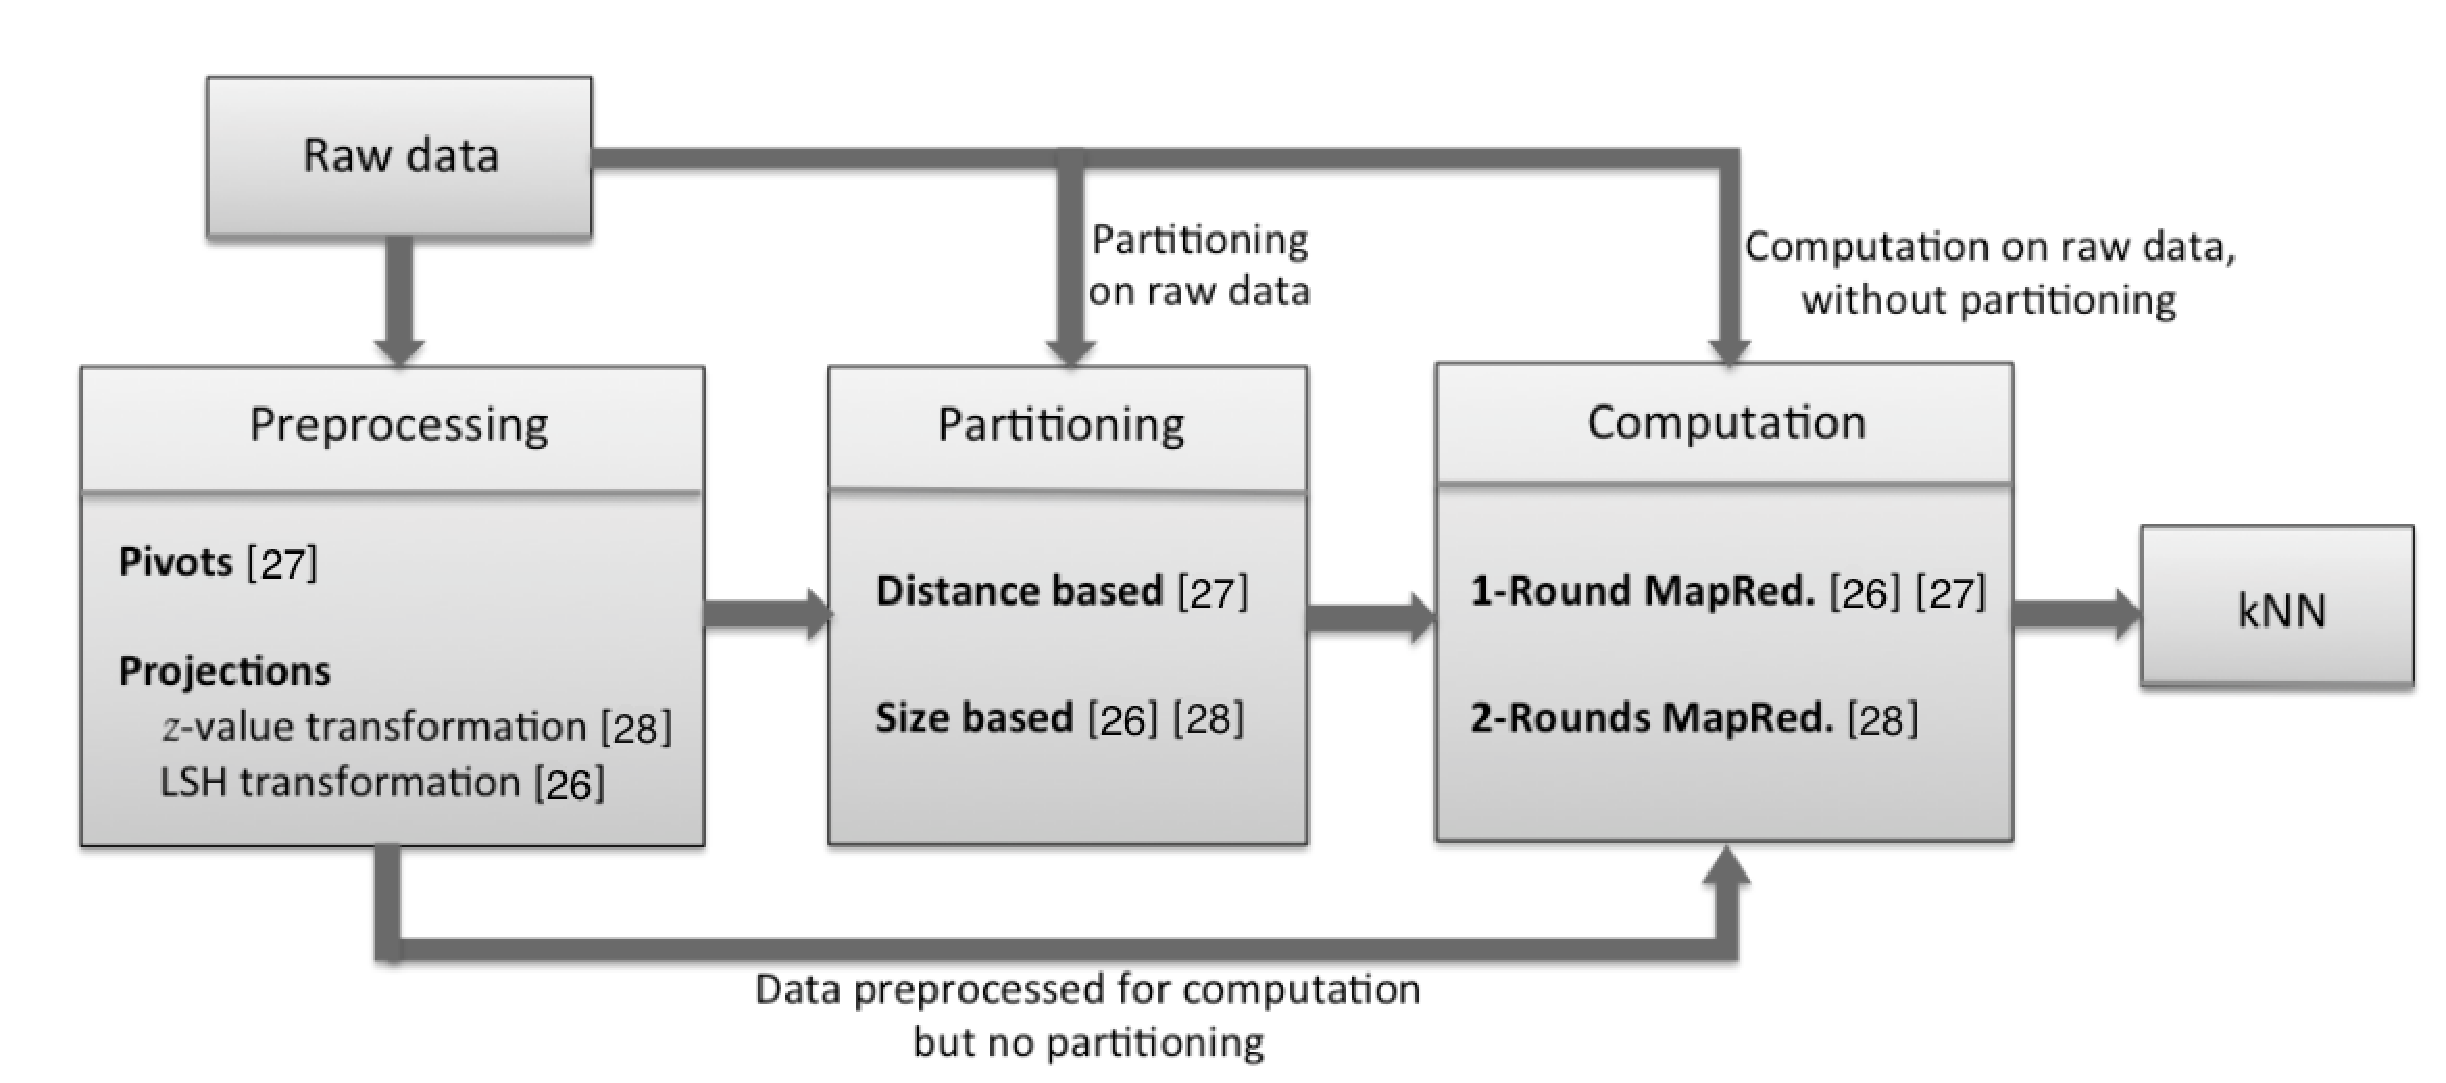
\includegraphics{res/workflow.pdf}}
\caption{Usual workflow of a kNN computation using MapReduce \label{workflow}}
\end{figure*}
Figure~\ref{workflow} summarizes the 
workflow we have gone through in this section and the techniques associated with each step.

%\begin{figure*}[t]
%\center
%\scalebox{0.35}{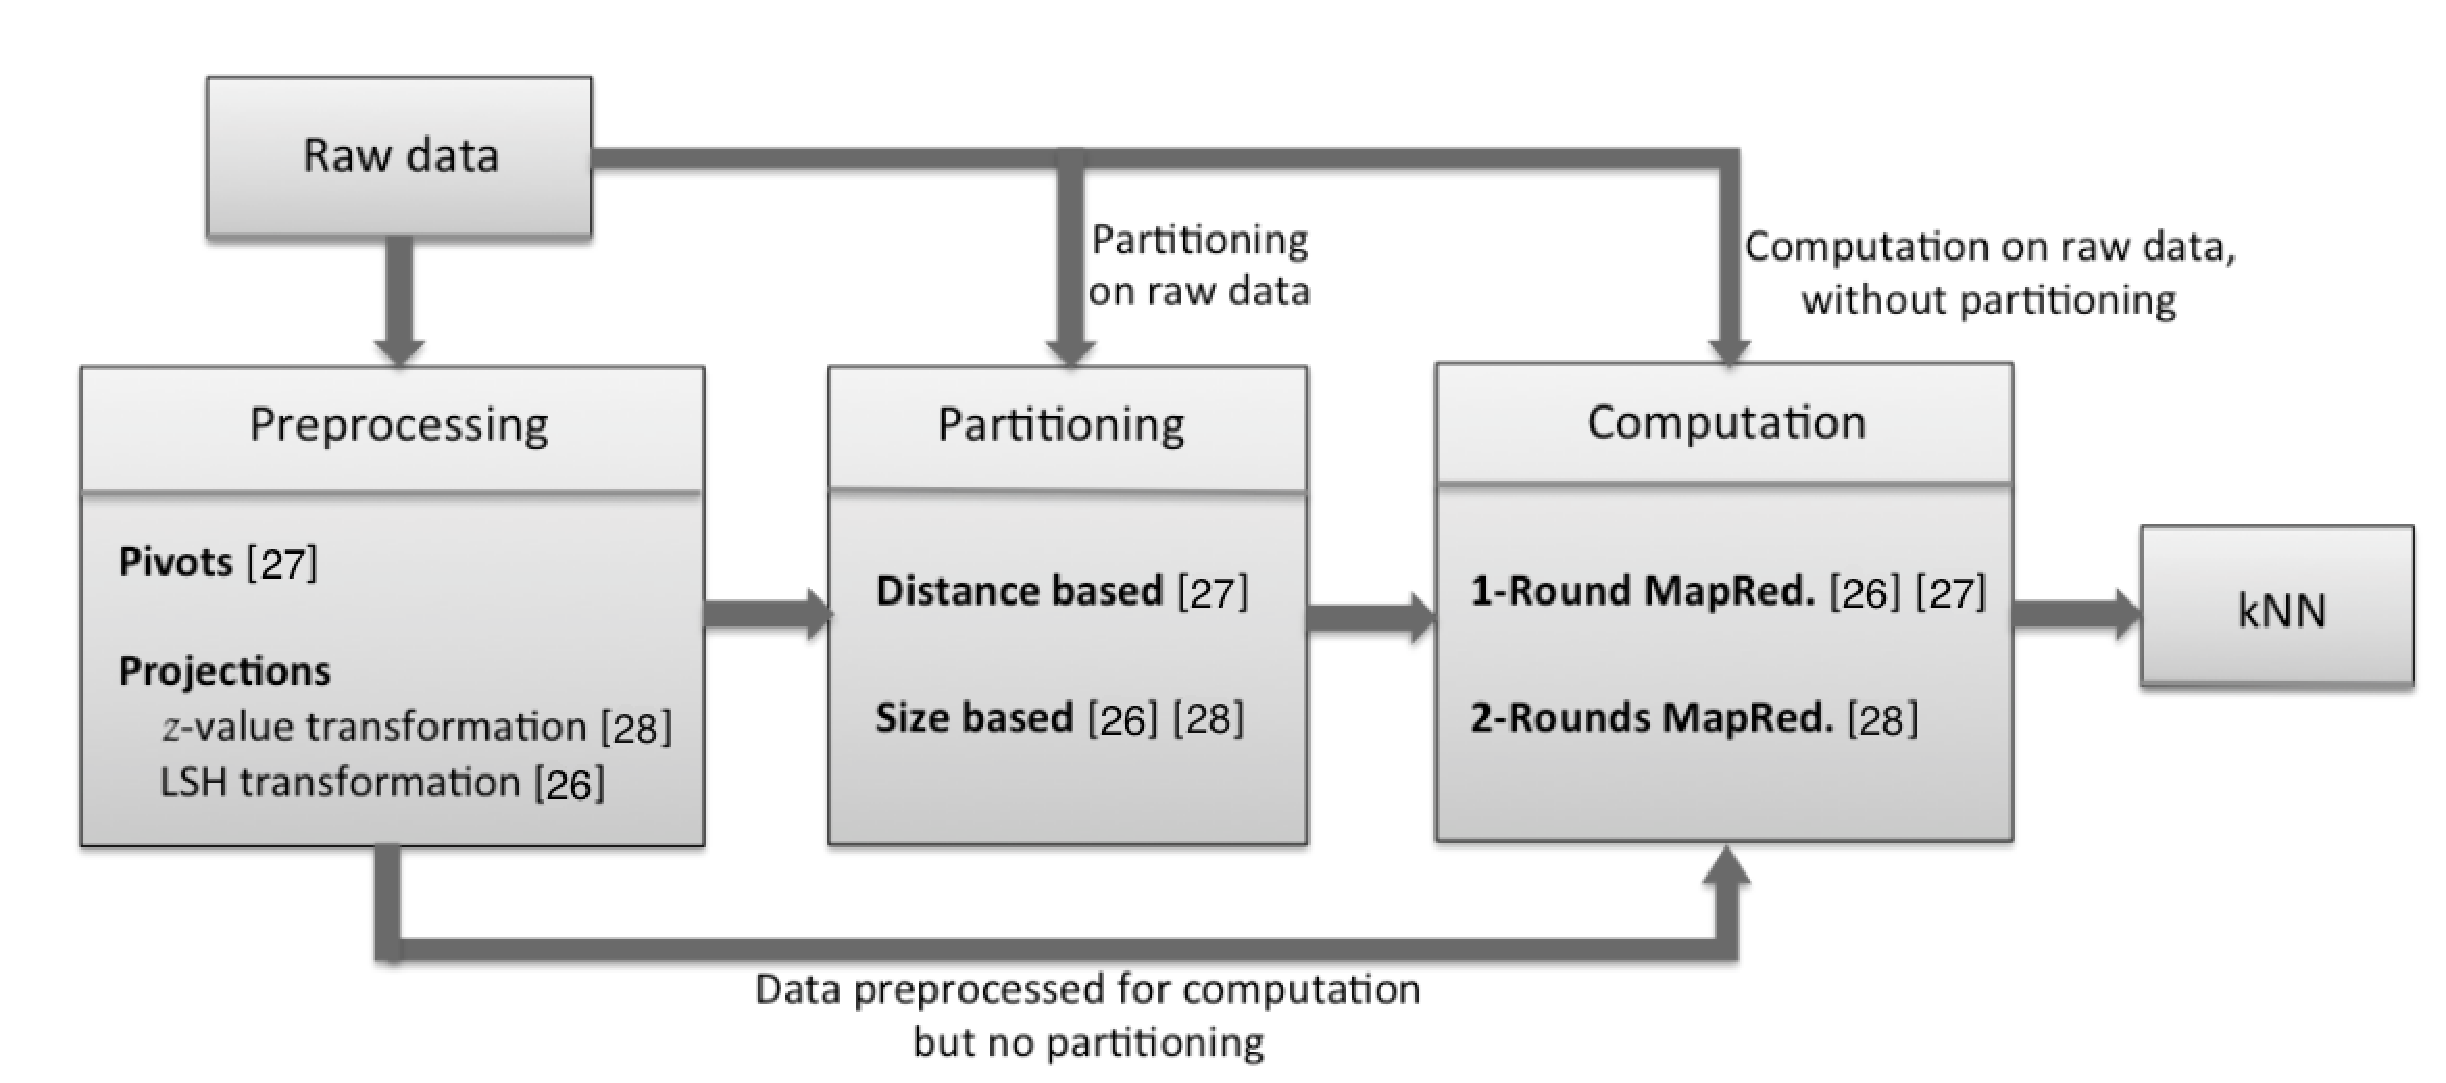
\includegraphics{res/workflow.pdf}}
%\caption{Usual workflow of a kNN computation using MapReduce \label{workflow}}
%\end{figure*}
